%Note di Ingegneria del Software
%Sommario: Architettura, Coesione, Accoppiamento, Fan{in-out}, design pattern architetturali

\cornell{Ancora sulle qualità di una buona architettura}{ \begin{description}
\item [Flessibilità] Permette, al variare dei requisiti, di fare modifiche con costi contenuti
\item [Riusabilità] Le sue parti possono essere usate (utilmente) in altre applicazioni (in futuro)
\item [Efficienza] nel tempo, nello spazio, nelle comunicazioni (fra le parti)
\item [Affidabilità] Se un modulo fallisce non perdo il lavoro fatto
\item [Disponibilità] Vi è poco (o nessun) tempo di indisponibilità a causa di manutenzione (non tutto il sistema deve essere interrotto se qualche parte finisce sotto manutenzione)
\item [Safety] Resiste ai malfunzionamenti/Esente da malfunzionamenti gravi
\item [Security] Sicurezza rispetto alle intrusioni
\item [Semplicità] All'interno dell'architettura vi è solo il necessario e nulla di superfluo (meglio avere soluzioni semplici che non complesse)
\item [Incapsulazione] Non esporre l'esterno ad informazioni non utili, così da poter cambiare l'interno senza dover cambiare l'interfaccia (Information Hiding)
\item [Coesione] Dentro il modulo stanno cose che perseguono lo stesso obiettivo. Se manca una parte, il modulo risulta incompleto
\item [Basso Accoppiamento] Le parti dipendono poco o nulla tra di loro
\end{description}}

\cornell{Information Hiding}{Le componenti sono come delle "scatole nere" ed i clienti ne conoscono solo l'interfaccia.\\
I funzionamenti interni delle componenti sono nascosti.\\
L'Information Hiding comporta alcuni benefici: \begin{itemize}
\item L'esterno non può fare assunzioni sull'interno delle componenti
\item Vi è una migliore manutenibilità
\item Si hanno meno dipendenze ed aumentano le possibilità di riuso
\end{itemize}}

\cornell{Coesione}{Le Funzionalità "vicine" devono stare nella stessa componente.\\
Ogni componente che sta in un modulo ha un motivo valido per starci.\\
Ha forti legami con il principio SOLID.}
\cornell{Tipi di Coesione Buona}{ \begin{itemize}
\item Funzionale
\item Sequenziale
\item Informativa
\end{itemize}\\
Ma su tutte prevale quella che persegue l'Information Hiding}

\cornell{Accoppiamento}{Dipendenza reciproca "cattiva".\\
Si viene a creare: \begin{itemize}
\item Facendo assunzioni sull'interno di certe cose (dall'esterno di tali)
\item Imponendo, dall'esterno, vincoli sull'interno di una componente
\item Condividendo frammenti di risorse
\end{itemize}\\
L'accoppiamento deve essere quanto più possibile minimizzato, ma non può essere portato a zero.}
\cornell{Misurare L'accoppiamento}{Considerando: \[U= \text{utilizzo reciproco di M componenti}\]
Possiamo vedere che \[ U = \begin{cases}
0 \text{ come valore minimo}\\
M \times M \text{ come valore massimo}
\end{cases} \]
Possiamo dire che più un modulo viene chiamato, più questo può essere considerato utile. Chiamiamo questa misura "indice di utilità" o "fan-in" ($SFIN$)\\
Mentre più un modulo fa uso di altri pezzi, più alta è la sua dipendenza da altri, chiamiamo questa misura "indice di dipendenza" o "fan-out" ($SFOUT$)\\
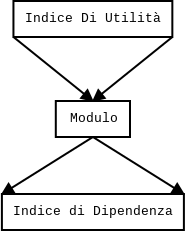
\includegraphics[scale=0.7]{images/33.png}}
\cornell{Riuso}{Tramite riuso si capitalizzano sottosistemi già esistenti: \begin{itemize}
\item Impiegandolì per più prodotti
\item Ottenendo un minor costo realizzativo (sono già fatti)
\item Ottenendo un minor costo di verifica (sono già testati e verificati)
\end{itemize}\\
È possibile \begin{itemize}
\item Progettare \textbf{per} riuso (Più complesso, dato che bisogna riuscire ad anticipare i bisogni futuri)
\item Progettare \textbf{con} riuso (Minimizzando le modifiche alle componenti riusate, altrimenti si perde il valore del riuso stesso.)
\end{itemize}\\
Costo puro nel breve periodo, risparmio nel medio termine (quindi può essere classificato come un investimento)}

\cornell{Progettazione Architetturale}{Tre stili: \begin{itemize}
\item Top-Down (Stile funzionale)
\item Bottom-Up (Stile Object-Oriented)
\item Meet-in-The-Middle: Approccio intermedio / misto.\\È quello usato più di frequente
\end{itemize}}

\cornell{Framework}{Insieme integrato di componenti software prefabbricate:\\
Prima della programmazione object-oriented erano detti librerie.\\
Possono essere classificate (secondo la progettazione architetturale): \begin{itemize}
\item Come Bottom-Up, dato che il codice è già sviluppato
\item Come Top-Down perchè impongono uno stile architetturale più o meno specifico.
\end{itemize}\\
I framework sono molto utili come base riusabile di diverse applicazioni in un dato dominio.\\
Un esempio di framework può essere Swing, usato per le GUI in Java.}
\cornell{Pattern}{Un pattern è uno stile o una serie di elementi ricorrenti in un'architettura.}

\cornell{Design Pattern Architetturali}{Soluzioni progettuali a problemi ricorrenti.\\
Un paio di esempi di design pattern architetturali possono essere: \begin{description}
\item [Architettura Multilivello] In cui ogni strato conosce e comunica solo con gli strati adiacenti (Ad esempio in ISO/OSI o TCP/IP)\\
Un esempio di architettura multilivello è l'architettura "three-tier", composta da: \begin{itemize}
\item Interfaccia Utente
\item Logica di Applicazione
\item Modello dei dati e persistenza
\end{itemize}
\item [Architettura Model-View-Controller]
\end{description}}

\cornell{Progettazione di dettaglio: Attività}{Definizione delle \textbf{unità} realizzative (moduli), con l'obiettivo di ottenere specifiche da dare ai programmatori.\\
Successivamente si attua una specifica delle unità come moduli (a seconda delle caratteristiche del linguaggio utilizzato)}

\cornell{Progettazione di Dettaglio: Obiettivi}{ \begin{itemize}
\item Definire le unità architetturali allo scopo di realizzare le componenti dell'architettura logica
\item Produrre la documentazione necessaria alla specifica di ogni unità (la cui struttura può seguire quella consigliata nello standard IEEE 1016:1998)
\item Definire gli strumenti per le prove di unità (come casi di prova e componenti ausiliarie per verifiche di integrazione)
\end{itemize}}
\cornell{Stati di progresso secondo SEMAT}{ \begin{description}
\item [Architecture Selected] Ho pensato all'architettura, al riuso, alle decisioni su make/buy/build
\item [Demonstrable] So enunciare e difendere (dimostrare) le proprietà buone della mia architettura
\item [Usable] Il Sistema è utilizzabile e la quantità di difetti residui è accettabile.
\item [Ready] La documentazione per l'utente è pronta e gli stakeholder vogliono che il prodotto divenga operativo
\end{description} }
